\section{TPM} % Multiple attack has been found - ref articles in bib
The Trusted Platform Module (TPM) is a specialised chip that stores RSA encryption keys specific for the host system for hardware authentication. It is used as a component on an endpoint device and is used for the Windows BitLocker.
The TPM contains an RSA key pair of the Endorsement Key (EK) and the owner-specified password. When a user takes ownership of the TPM, a \textit{Storage Root Key} (SRK) is generated. The SRK works as the root of a tree like structure, where future keys are stored, by which are used for encrypting data. To each TPM key a 160-bit string is associated called the \textit{authdata}, and works like a password to authorise the use of a key. \\ \\

\subsection{The API and its commands}
The API offers operations related to; \textit{Secure key management and storage}, which generates new key and impose restrictions on their use; \textit{Platform configuration registers (PCR)} which stores hashes of measurements taken by external software and later lock those by signing them with a specified key. This allows for the TPM to provide \textit{root of trust} for a variety of applications such as:
\begin{itemize}
	\item \textit{Secure storage}: allows the user to securely store content which is encrypted with a key only available to the TPM
	\item \textit{Platform authentication}: a platform can obtain keys by which it can authenticate itself reliably (rewrite)
	\item \textit{Platform measurement and reporting}: A platform can create reports of its integrity and configuration state that can be relied on by a remote verifier (rewirte)
\end{itemize}
The TPM's application program interface (API) offers a wide variety of commands, that e.g. allow the user to load new keys or certify a key by another one. As the TPM offers more than 90 different commands through its application program interface (API), the report will only focus on a small sample of these. Each command has to be called inside an \textit{authorisation session}, so the user will first have to choose between one of the following sessions:
\begin{itemize}
  \item Object Independent Authorisation Protocol (OIAP)
  \item Object Specific Authorisation Protocol (OSAP)
\end{itemize}
The OIAP creates a session that can manipulate any object, but will only work with certain commands. When setting up the session, the TPM will send back a \textit{session handle} and a fresh \textit{even nonce} as part of its arguments. 
The OSAP creates a session that can only manipulate a specific object, specified at the session start, so when starting the session, the user will have to send with it the \textit{key handle} of the object and an \textit{odd nonce}. \\
This rotation of nonces, with the user's defined as \textit{odd nonces} and the TPM's as \textit{even nonce}, guarantees freshness of the commands and responses, which are then encrypted with an HMAC and works as a \textit{shared secret} hmac($auth, \langle Ne^{OSAP}, No^{OSAP} \rangle $). \\ \\

\subsection{Example of commands}
To illustrate the exchange of message between the TPM and a user, three commands besides the OIAP and OSAP has been chosen to get a better look at the authorisation going on:
\begin{itemize}
	\item \textit{TPM\_CreateWrapKey}: Creates a new key in the storage key tree
	\item \textit{TPM\_LoadKey2}: Load key from tree into the TPM internal memory
	\item \textit{TPM\_Seal}: Uses key to encrypt data
\end{itemize}
TODO: describe pkh!
In the following illustration, the user starts with creating an OSAP session with the TPM to generate a \textit{shared secret} = \textit{S}. \\ \\
\begin{center}
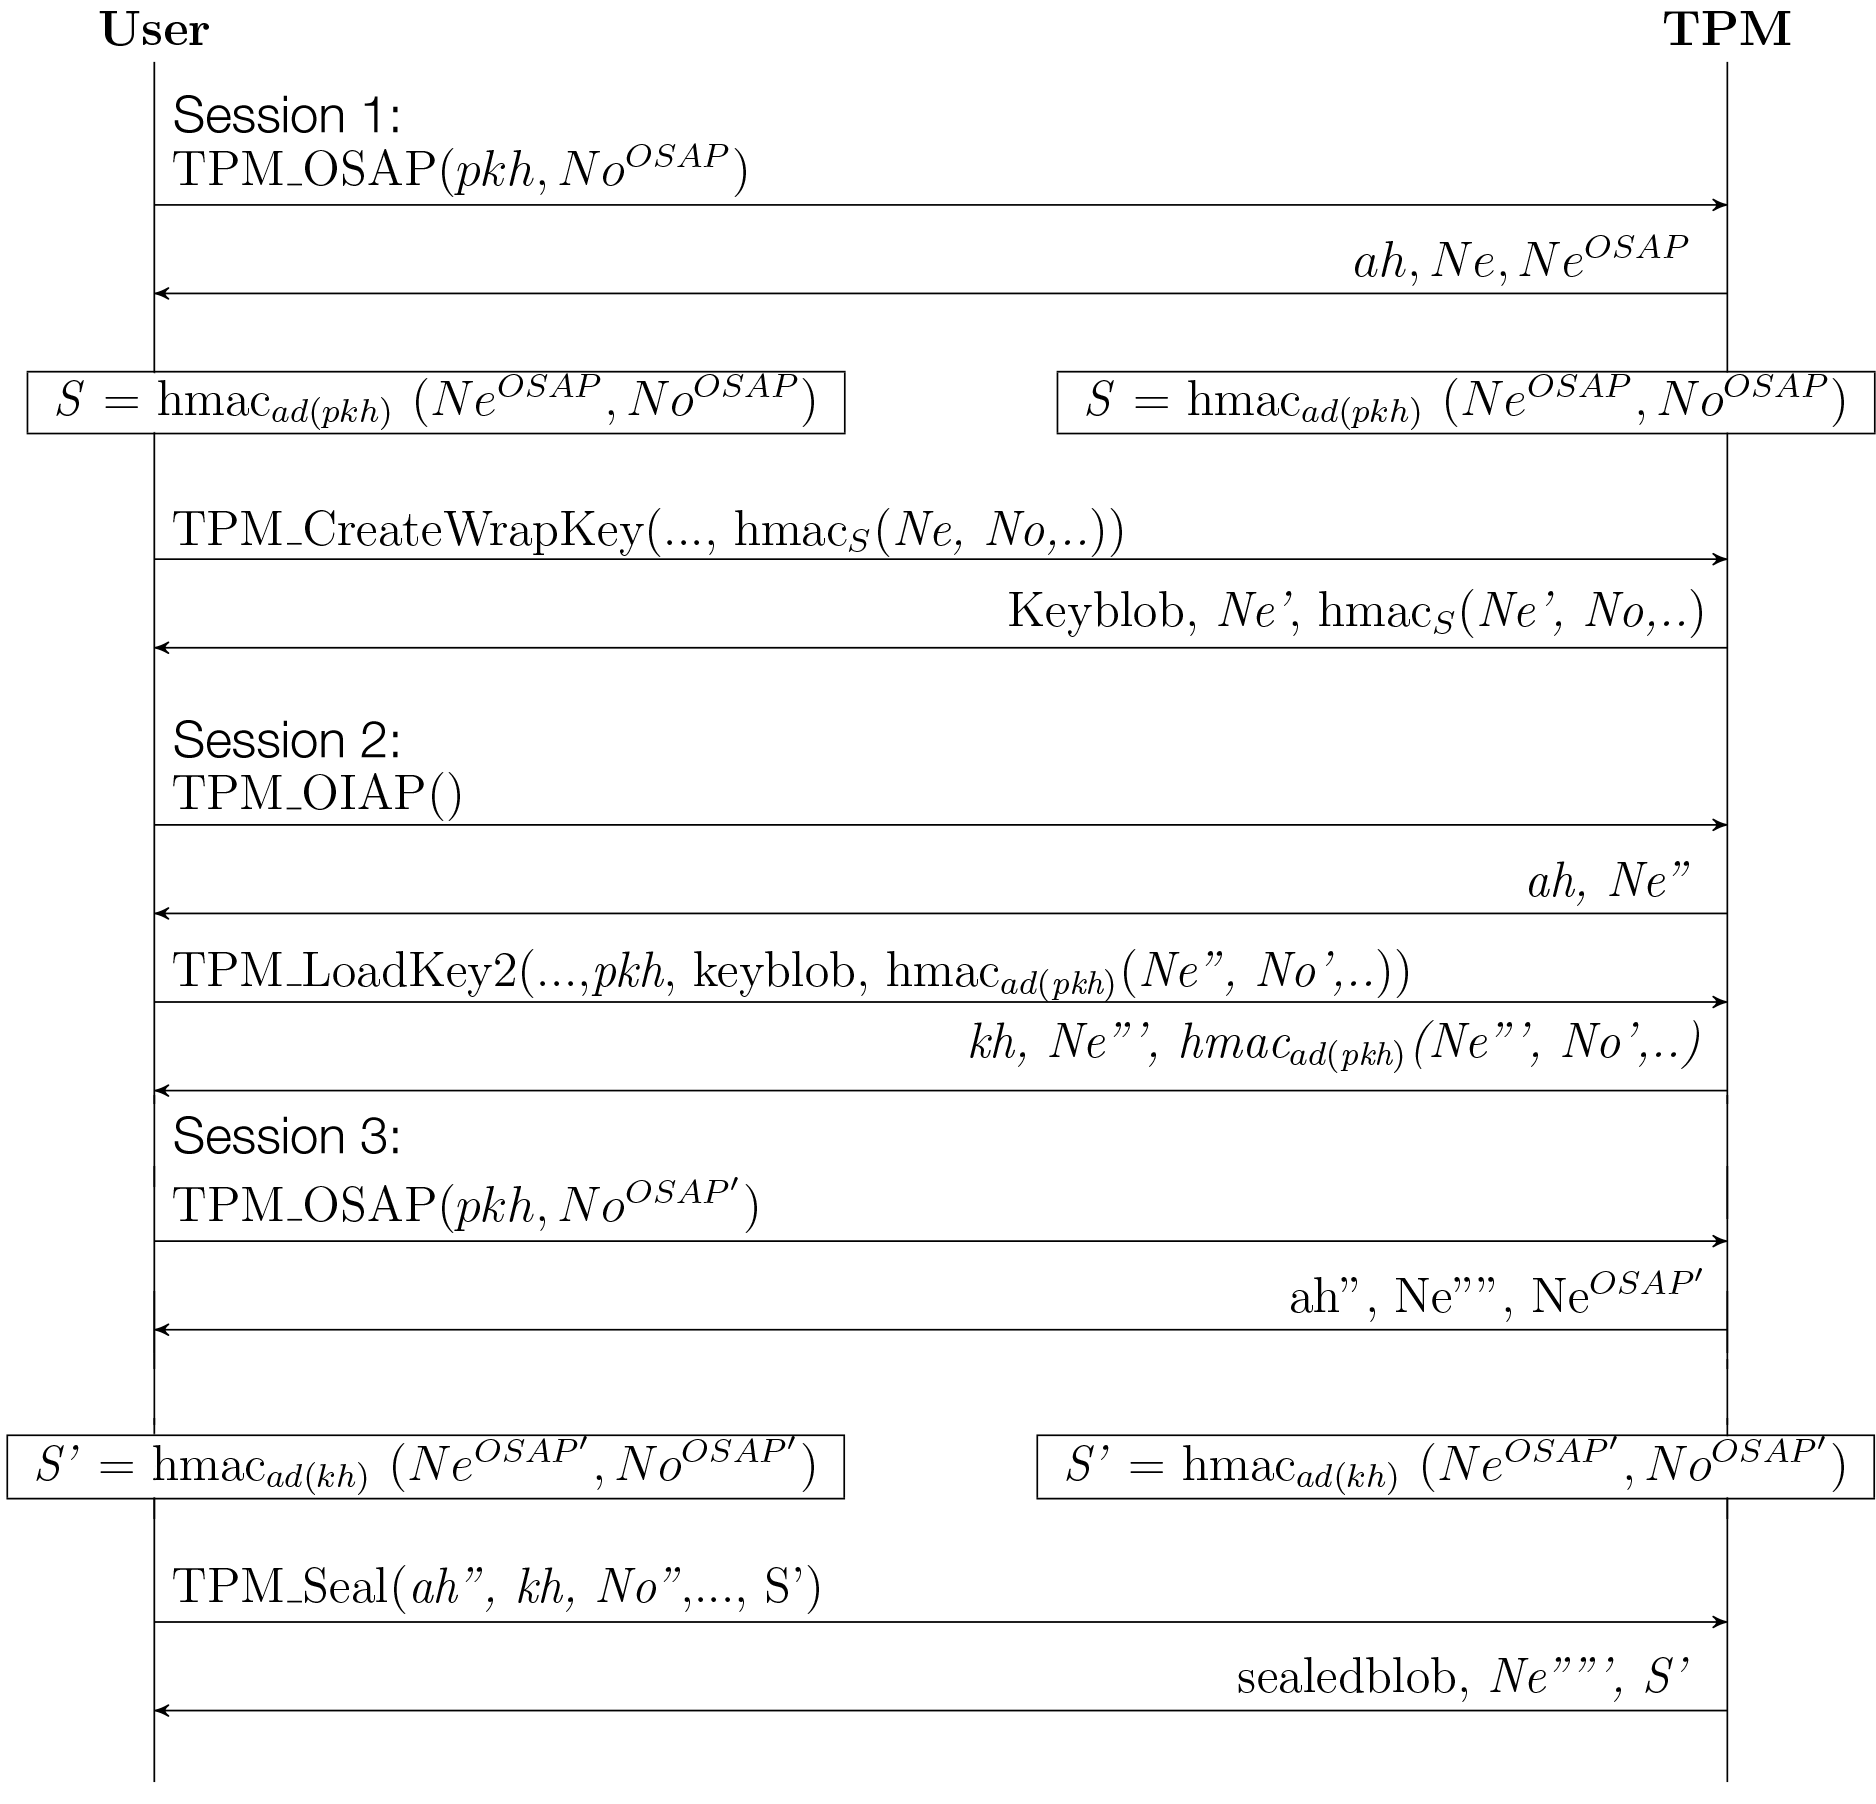
\includegraphics{Graphics/Diagram}
\end{center}
%\begin{center}
\begin{tikzpicture}[node distance=12cm,auto,>=stealth']
    \node[] (TPM) {\textbf{TPM}};
    \node[left = of TPM] (User) {\textbf{User}};
    \node[below of=TPM, node distance=15cm] (TPM_ground) {};
    \node[below of=User, node distance=15cm] (User_ground) {};
    %
    \draw (User) -- (User_ground); % horizontal lines
    \draw (TPM) -- (TPM_ground); % horizontal lines
    \draw[->] ($(User)!0.10!(User_ground)$) -- node[above,scale=1,near start]{\quad TPM\_OSAP($pkh, No^{OSAP}$)} ($(TPM)!0.10!(TPM_ground)$);
    \draw[<-] ($(User)!0.15!(User_ground)$) -- node[above,scale=1,near end]{$ah, Ne, Ne^{OSAP}$} ($(TPM)!0.15!(TPM_ground)$);
    \draw[->] ($(User)!0.30!(User_ground)$) -- node[above,scale=1,midway]{TPM\_CreateWrapKey(..., hmac$_S$(\textit{Ne, No,..}))} ($(TPM)!0.30!(TPM_ground)$);
    \draw[<-] ($(User)!0.35!(User_ground)$) -- node[above,scale=1,near end]{Keyblob, \textit{Ne'}, hmac$_S$(\textit{Ne', No,..})} ($(TPM)!0.35!(TPM_ground)$);
    \draw[->] ($(User)!0.45!(User_ground)$) -- node[above,scale=1,near start]{TPM\_OIAP()} ($(TPM)!0.45!(TPM_ground)$);
    \draw[<-] ($(User)!0.50!(User_ground)$) -- node[above,scale=1,near end]{\textit{ah, Ne''}} ($(TPM)!0.50!(TPM_ground)$);
    \draw[->] ($(User)!0.55!(User_ground)$) -- node[above,scale=1,midway]{TPM\_LoadKey2(...,\textit{pkh}, keyblob, hmac$_{ad(\textit{pkh})}$(\textit{Ne'', No',..}))} ($(TPM)!0.55!(TPM_ground)$);
    \draw[<-] ($(User)!0.60!(User_ground)$) -- node[above,scale=1,near end]{\textit{kh, Ne''', hmac$_{ad(\textit{pkh})}$(\textit{Ne''', No',..})}} ($(TPM)!0.60!(TPM_ground)$);
    \draw[->] ($(User)!0.65!(User_ground)$) -- node[above,scale=1,near start]{TPM\_OSAP($pkh, No^{OSAP'}$)} ($(TPM)!0.65!(TPM_ground)$);
    \draw[<-] ($(User)!0.70!(User_ground)$) -- node[above,scale=1,near end]{ah'', Ne'''', Ne$^{OSAP'}$} ($(TPM)!0.70!(TPM_ground)$);
    \draw[->] ($(User)!0.90!(User_ground)$) -- node[above,scale=1,near start]{TPM\_Seal(\textit{ah'', kh, No''},..., S')} ($(TPM)!0.90!(TPM_ground)$);
    \draw[<-] ($(User)!0.95!(User_ground)$) -- node[above,scale=1,near end]{sealedblob, \textit{Ne''''', S'}} ($(TPM)!0.95!(TPM_ground)$);
\end{tikzpicture}
\end{center}

\begin{tabular} { |c| }
\hline
\textit{S} = hmac$_{ad(pkh)}$ ($Ne^{OSAP}, No^{OSAP}$) \\ 
\hline
\end{tabular}
\\ \\
\begin{tabular} { |c| }
\hline
\textit{S'} = hmac$_{ad(kh)}$ ($Ne^{OSAP'}, No^{OSAP'}$) \\ 
\hline
\end{tabular}


\iffalse
    \draw[->] ($(User)!0.25!(User_ground)$) -- node[above,scale=1,near start]{\quad TPM\_OSAP($pkh, No^{OSAP}$)} ($(TPM)!0.25!(TPM_ground)$);
    \draw[<-] ($(User)!0.35!(User_ground)$) -- node[above,scale=1,near end]{$ah, Ne, Ne^{OSAP}$} ($(TPM)!0.35!(TPM_ground)$);
    \draw[->] ($(User)!0.45!(User_ground)$) -- node[above,scale=1,near start]{TPM\_CreateWrapKey(...)} ($(TPM)!0.45!(TPM_ground)$);
    \draw[<-] ($(User)!0.55!(User_ground)$) -- node[above,scale=1,near end]{Keyblob} ($(TPM)!0.55!(TPM_ground)$);
    \draw[->] ($(User)!0.75!(User_ground)$) -- node[above,scale=1,near start]{TPM\_OIAP()} ($(TPM)!0.75!(TPM_ground)$);
    \draw[<-] ($(User)!0.85!(User_ground)$) -- node[above,scale=1,near end]{ah, ne} ($(TPM)!0.85!(TPM_ground)$);
    \draw[->] ($(User)!0.95!(User_ground)$) -- node[above,scale=1,near start]{TPM\_LoadKey2} ($(TPM)!0.95!(TPM_ground)$);
    \draw[<-] ($(User)!1.05!(User_ground)$) -- node[above,scale=1,near end]{Kh, ne, hmac(..)} ($(TPM)!1.05!(TPM_ground)$);
    \draw[->] ($(User)!1.25!(User_ground)$) -- node[above,scale=1,near start]{TPM\_OSAP(...)} ($(TPM)!1.25!(TPM_ground)$);
    \draw[<-] ($(User)!1.35!(User_ground)$) -- node[above,scale=1,near end]{ah, ne, ne} ($(TPM)!1.35!(TPM_ground)$);
    \draw[->] ($(User)!1.55!(User_ground)$) -- node[above,scale=1,near start]{TPM\_Seal(...)} ($(TPM)!1.55!(TPM_ground)$);
    \draw[<-] ($(User)!1.65!(User_ground)$) -- node[above,scale=1,near end]{sealedblob} ($(TPM)!1.65!(TPM_ground)$);
\fi 

%Examples of TPM commands with applied pi-calculus ?

%Note: remote attestation